\begin{center}
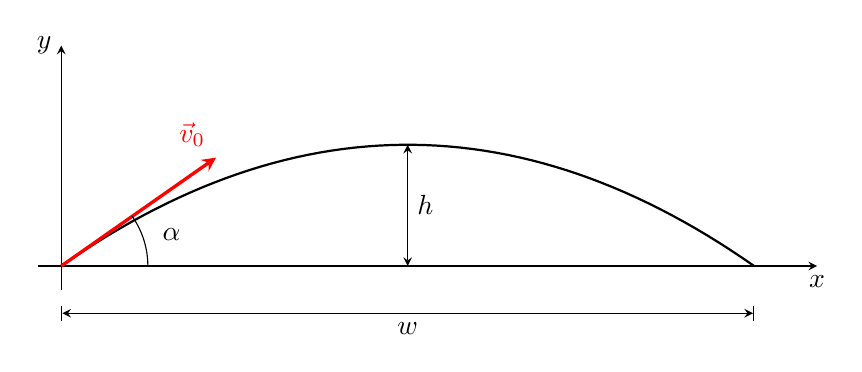
\begin{tikzpicture}[>=stealth]
 \draw[->] (-0.3,0) -- (9.6,0) node[below] {$x$};
 \draw[->] (0,-0.3) -- (0,2.8) node[left] {$y$};
 \draw[thick, domain=0:8.8, samples=60] plot (\x, {6.16*\x*(8.8-\x)/77.44});
 \draw[->, very thick, red] (0,0) -- (35:2.4) node[above left] {$\vec v_0$};
 \draw (1.1,0) arc (0:35:1.1);
 \node at (1.4,0.4) {$\alpha$};
 \draw[<->] (4.4,0) -- (4.4,1.54) node[midway, right] {$h$};
 \draw[|<->|] (0,-0.6) -- (8.8,-0.6) node[midway, below] {$w$};
\end{tikzpicture}
\end{center}

Die Teilgeschwindigkeiten beim Abstoss sind $v_x = v_0\cos\alpha$ (horizontal, bleibt konstant) und $v_y = v_0\sin\alpha$ (vertikal, nimmt gleichmässig ab). Im höchsten Punkt ist die vertikale Geschwindigkeit null; die Steigzeit ist $t_\text{s} = v_y/g$, die mittlere vertikale Geschwindigkeit beim Steigen $v_y/2$. Damit ist die Wurfhöhe
\begin{align}
 h &= \frac{v_y}{2}\cdot t_\text{s} = \frac{v_y^2}{2g} = \hmaxF \\
   &= \frac{\left(\vf\cdot\sin\left(\alO\right)\right)^2}{2\cdot\gE} \\
   &= \hmax \approx \result{\hmaxP{0}{2}}
\end{align}
Die Flugzeit ist $2t_\text{s}$ (Abstoss und Landung auf gleicher Höhe), die Wurfweite
\begin{align}
 w &= v_x\cdot 2t_\text{s} = \frac{2v_xv_y}{g} = \xwF \\
   &= \frac{2\cdot\left(\vf\right)^2\cdot\sin\left(\alO\right)\cdot\cos\left(\alO\right)}{\gE} \\
   &= \xw \approx \result{\xwP{0}{2}}
\end{align}
Der Luftwiderstand ist vernachlässigt; ein echter Fussball fliegt weniger hoch und weniger weit.
